% Options for packages loaded elsewhere
\PassOptionsToPackage{unicode}{hyperref}
\PassOptionsToPackage{hyphens}{url}
%
\documentclass[
]{article}
\usepackage{amsmath,amssymb}
\usepackage{lmodern}
\usepackage{ifxetex,ifluatex}
\ifnum 0\ifxetex 1\fi\ifluatex 1\fi=0 % if pdftex
  \usepackage[T1]{fontenc}
  \usepackage[utf8]{inputenc}
  \usepackage{textcomp} % provide euro and other symbols
\else % if luatex or xetex
  \usepackage{unicode-math}
  \defaultfontfeatures{Scale=MatchLowercase}
  \defaultfontfeatures[\rmfamily]{Ligatures=TeX,Scale=1}
\fi
% Use upquote if available, for straight quotes in verbatim environments
\IfFileExists{upquote.sty}{\usepackage{upquote}}{}
\IfFileExists{microtype.sty}{% use microtype if available
  \usepackage[]{microtype}
  \UseMicrotypeSet[protrusion]{basicmath} % disable protrusion for tt fonts
}{}
\makeatletter
\@ifundefined{KOMAClassName}{% if non-KOMA class
  \IfFileExists{parskip.sty}{%
    \usepackage{parskip}
  }{% else
    \setlength{\parindent}{0pt}
    \setlength{\parskip}{6pt plus 2pt minus 1pt}}
}{% if KOMA class
  \KOMAoptions{parskip=half}}
\makeatother
\usepackage{xcolor}
\IfFileExists{xurl.sty}{\usepackage{xurl}}{} % add URL line breaks if available
\IfFileExists{bookmark.sty}{\usepackage{bookmark}}{\usepackage{hyperref}}
\hypersetup{
  pdftitle={Important Penguin Analysis},
  hidelinks,
  pdfcreator={LaTeX via pandoc}}
\urlstyle{same} % disable monospaced font for URLs
\usepackage[margin=1in]{geometry}
\usepackage{color}
\usepackage{fancyvrb}
\newcommand{\VerbBar}{|}
\newcommand{\VERB}{\Verb[commandchars=\\\{\}]}
\DefineVerbatimEnvironment{Highlighting}{Verbatim}{commandchars=\\\{\}}
% Add ',fontsize=\small' for more characters per line
\usepackage{framed}
\definecolor{shadecolor}{RGB}{248,248,248}
\newenvironment{Shaded}{\begin{snugshade}}{\end{snugshade}}
\newcommand{\AlertTok}[1]{\textcolor[rgb]{0.94,0.16,0.16}{#1}}
\newcommand{\AnnotationTok}[1]{\textcolor[rgb]{0.56,0.35,0.01}{\textbf{\textit{#1}}}}
\newcommand{\AttributeTok}[1]{\textcolor[rgb]{0.77,0.63,0.00}{#1}}
\newcommand{\BaseNTok}[1]{\textcolor[rgb]{0.00,0.00,0.81}{#1}}
\newcommand{\BuiltInTok}[1]{#1}
\newcommand{\CharTok}[1]{\textcolor[rgb]{0.31,0.60,0.02}{#1}}
\newcommand{\CommentTok}[1]{\textcolor[rgb]{0.56,0.35,0.01}{\textit{#1}}}
\newcommand{\CommentVarTok}[1]{\textcolor[rgb]{0.56,0.35,0.01}{\textbf{\textit{#1}}}}
\newcommand{\ConstantTok}[1]{\textcolor[rgb]{0.00,0.00,0.00}{#1}}
\newcommand{\ControlFlowTok}[1]{\textcolor[rgb]{0.13,0.29,0.53}{\textbf{#1}}}
\newcommand{\DataTypeTok}[1]{\textcolor[rgb]{0.13,0.29,0.53}{#1}}
\newcommand{\DecValTok}[1]{\textcolor[rgb]{0.00,0.00,0.81}{#1}}
\newcommand{\DocumentationTok}[1]{\textcolor[rgb]{0.56,0.35,0.01}{\textbf{\textit{#1}}}}
\newcommand{\ErrorTok}[1]{\textcolor[rgb]{0.64,0.00,0.00}{\textbf{#1}}}
\newcommand{\ExtensionTok}[1]{#1}
\newcommand{\FloatTok}[1]{\textcolor[rgb]{0.00,0.00,0.81}{#1}}
\newcommand{\FunctionTok}[1]{\textcolor[rgb]{0.00,0.00,0.00}{#1}}
\newcommand{\ImportTok}[1]{#1}
\newcommand{\InformationTok}[1]{\textcolor[rgb]{0.56,0.35,0.01}{\textbf{\textit{#1}}}}
\newcommand{\KeywordTok}[1]{\textcolor[rgb]{0.13,0.29,0.53}{\textbf{#1}}}
\newcommand{\NormalTok}[1]{#1}
\newcommand{\OperatorTok}[1]{\textcolor[rgb]{0.81,0.36,0.00}{\textbf{#1}}}
\newcommand{\OtherTok}[1]{\textcolor[rgb]{0.56,0.35,0.01}{#1}}
\newcommand{\PreprocessorTok}[1]{\textcolor[rgb]{0.56,0.35,0.01}{\textit{#1}}}
\newcommand{\RegionMarkerTok}[1]{#1}
\newcommand{\SpecialCharTok}[1]{\textcolor[rgb]{0.00,0.00,0.00}{#1}}
\newcommand{\SpecialStringTok}[1]{\textcolor[rgb]{0.31,0.60,0.02}{#1}}
\newcommand{\StringTok}[1]{\textcolor[rgb]{0.31,0.60,0.02}{#1}}
\newcommand{\VariableTok}[1]{\textcolor[rgb]{0.00,0.00,0.00}{#1}}
\newcommand{\VerbatimStringTok}[1]{\textcolor[rgb]{0.31,0.60,0.02}{#1}}
\newcommand{\WarningTok}[1]{\textcolor[rgb]{0.56,0.35,0.01}{\textbf{\textit{#1}}}}
\usepackage{longtable,booktabs,array}
\usepackage{calc} % for calculating minipage widths
% Correct order of tables after \paragraph or \subparagraph
\usepackage{etoolbox}
\makeatletter
\patchcmd\longtable{\par}{\if@noskipsec\mbox{}\fi\par}{}{}
\makeatother
% Allow footnotes in longtable head/foot
\IfFileExists{footnotehyper.sty}{\usepackage{footnotehyper}}{\usepackage{footnote}}
\makesavenoteenv{longtable}
\usepackage{graphicx}
\makeatletter
\def\maxwidth{\ifdim\Gin@nat@width>\linewidth\linewidth\else\Gin@nat@width\fi}
\def\maxheight{\ifdim\Gin@nat@height>\textheight\textheight\else\Gin@nat@height\fi}
\makeatother
% Scale images if necessary, so that they will not overflow the page
% margins by default, and it is still possible to overwrite the defaults
% using explicit options in \includegraphics[width, height, ...]{}
\setkeys{Gin}{width=\maxwidth,height=\maxheight,keepaspectratio}
% Set default figure placement to htbp
\makeatletter
\def\fps@figure{htbp}
\makeatother
\setlength{\emergencystretch}{3em} % prevent overfull lines
\providecommand{\tightlist}{%
  \setlength{\itemsep}{0pt}\setlength{\parskip}{0pt}}
\setcounter{secnumdepth}{-\maxdimen} % remove section numbering
\usepackage{amsmath}
\usepackage{booktabs}
\usepackage{caption}
\usepackage{longtable}
\ifluatex
  \usepackage{selnolig}  % disable illegal ligatures
\fi

\title{Important Penguin Analysis}
\author{}
\date{\vspace{-2.5em}}

\begin{document}
\maketitle

{
\setcounter{tocdepth}{2}
\tableofcontents
}
\begin{figure}
\centering
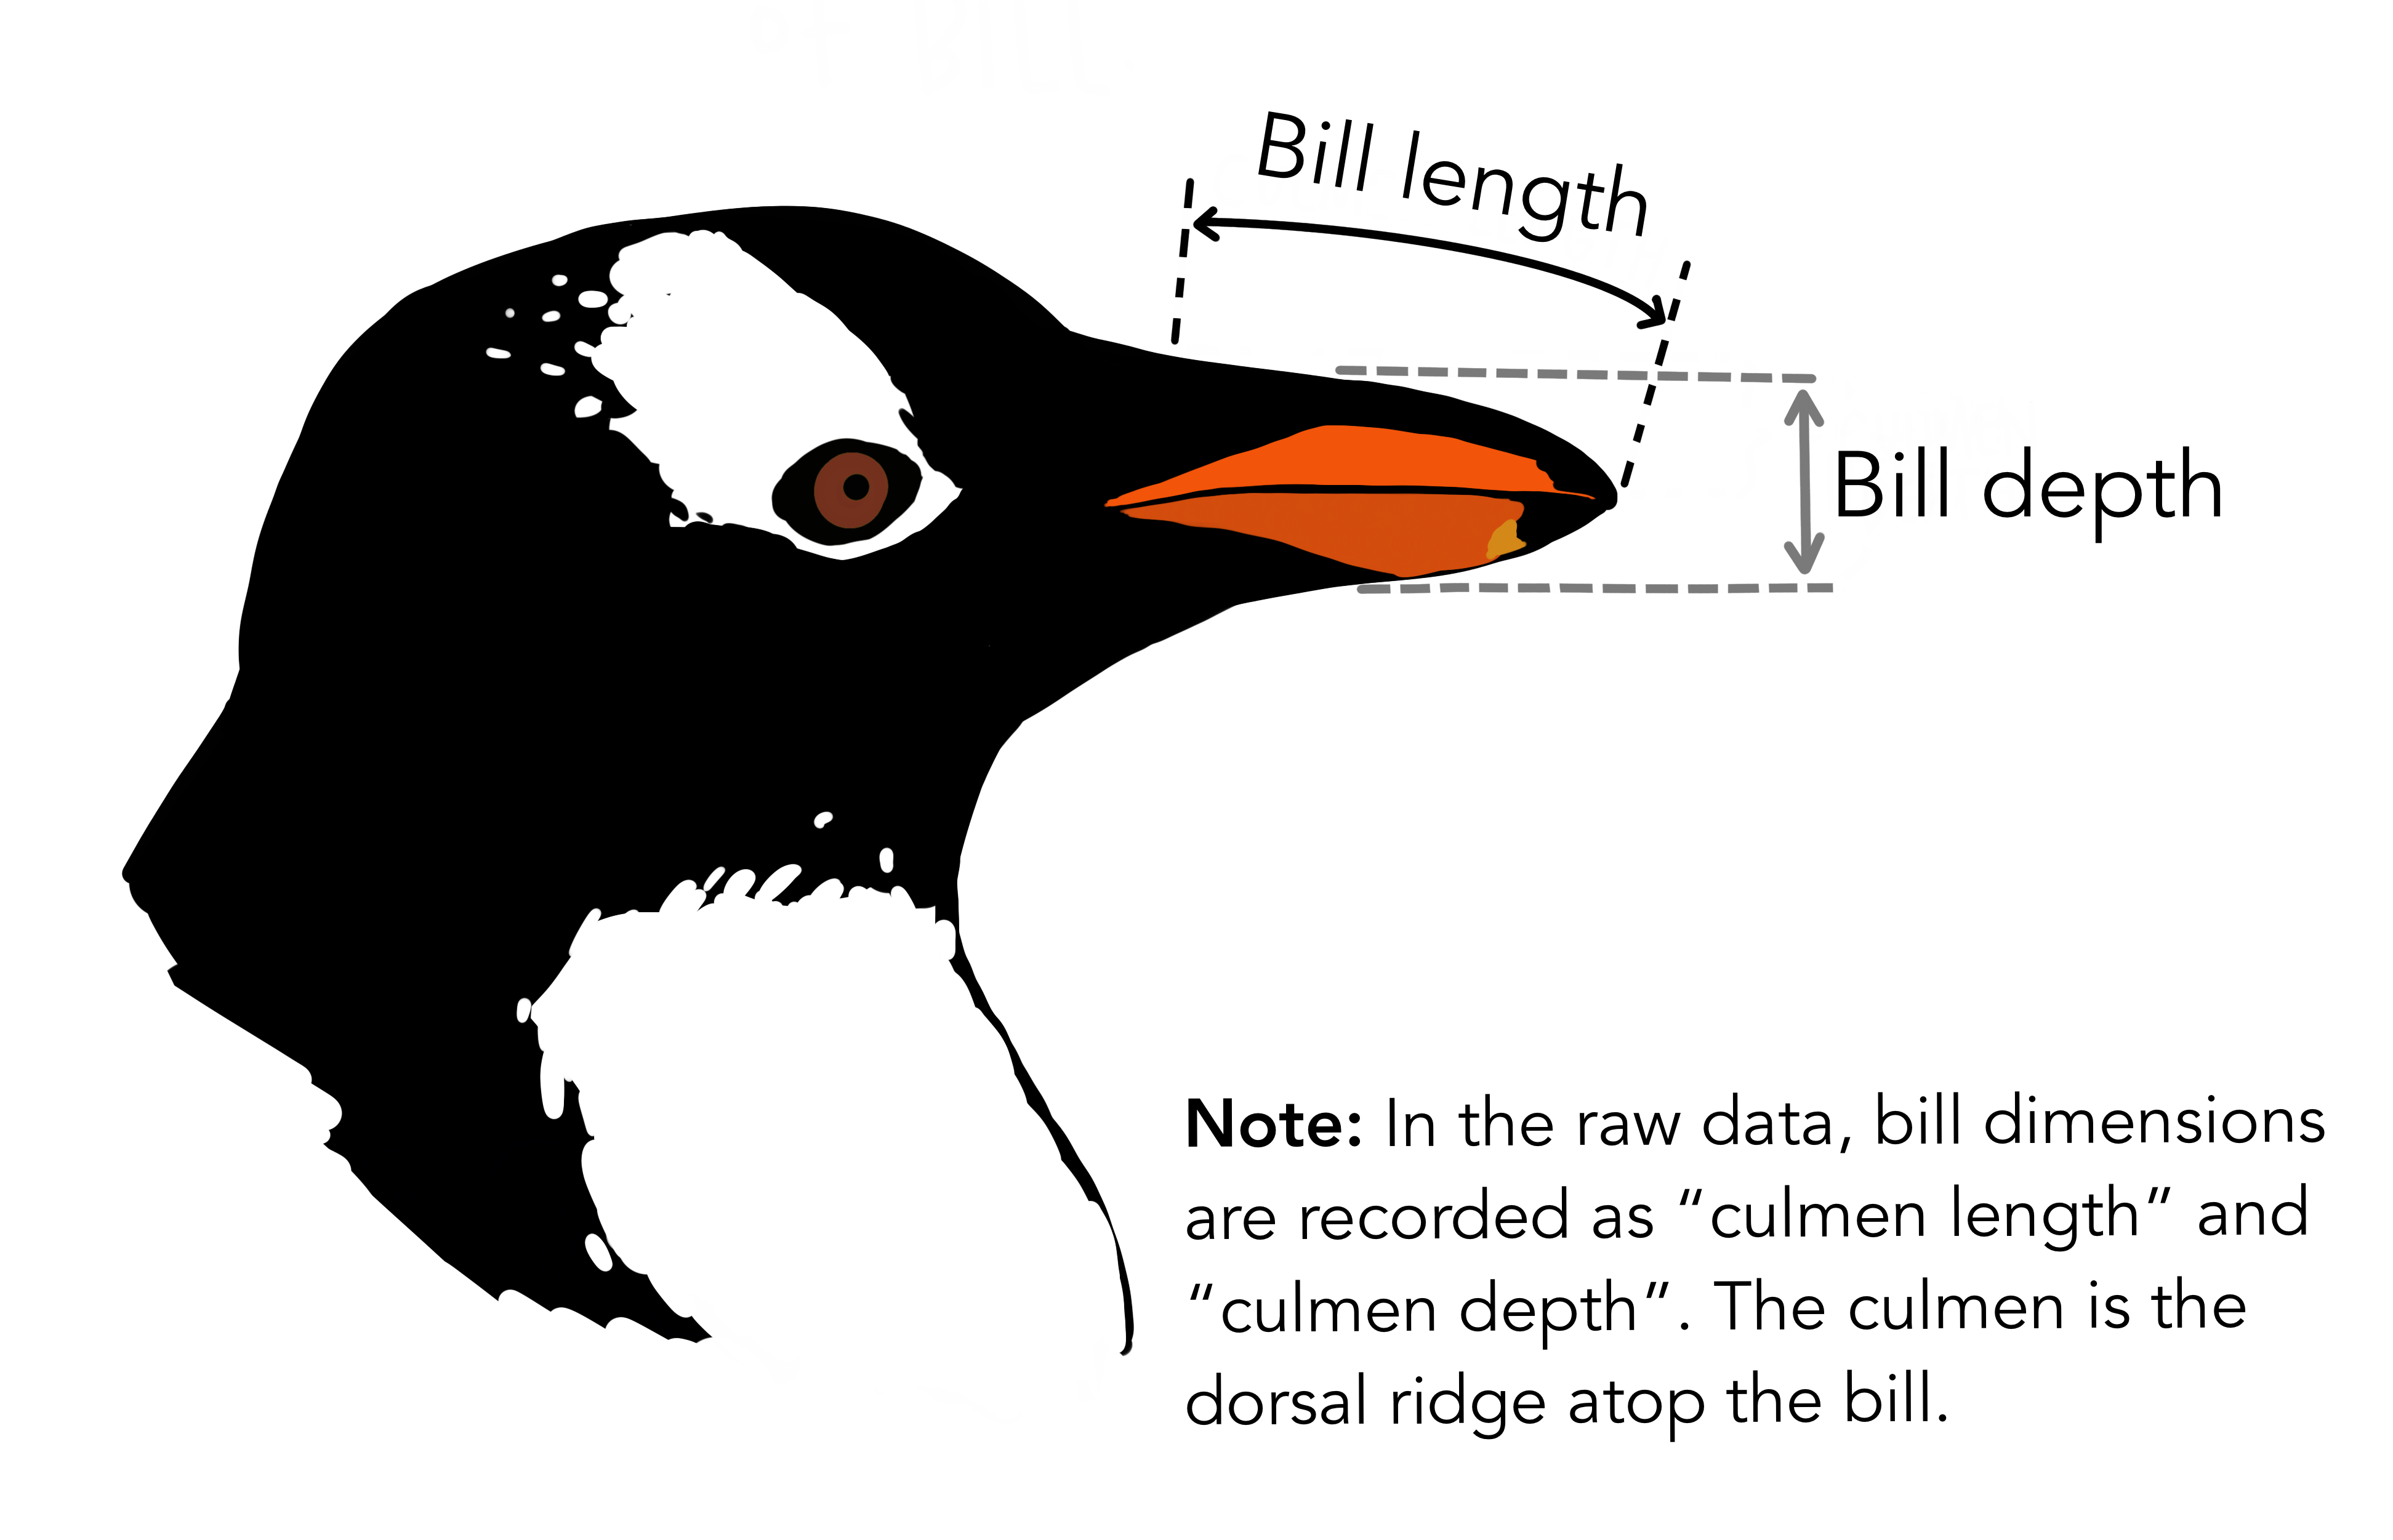
\includegraphics{culmen_depth.png}
\caption{Diagram of penguin head with indication of bill length and bill
depth.}
\end{figure}

\hypertarget{literate-programming}{%
\subsubsection{Literate Programming}\label{literate-programming}}

Per \href{https://en.wikipedia.org/wiki/Literate_programming}{Donald
Knuth}

\begin{quote}
A programming paradigm introduced by Donald Knuth in which a computer
program is given an explanation of its logic in a natural language, such
as English, interspersed with snippets of macros and traditional source
code, from which compilable source code can be generated.
\end{quote}

\hypertarget{initial-explore}{%
\subsubsection{Initial explore}\label{initial-explore}}

We can do a quick exploration of the data with \texttt{skimr::skim()}.
This will report the counts of various variables, along with some basic
descriptive statistics. The \texttt{skimr} package is fantastic for
quickly getting a sense of your datasets.

Ahead of \texttt{skimr} there are 344 penguins in this dataset, and the
unique species are Adelie, Gentoo, Chinstrap.

Per the \href{https://docs.ropensci.org/skimr/index.html}{rOpenSci
\texttt{skimr} docs}:

\begin{quote}
\texttt{skimr} provides a frictionless approach to summary statistics
which conforms to the principle of least surprise, displaying summary
statistics the user can skim quickly to understand their data. It
handles different data types and returns a skim\_df object which can be
included in a pipeline or displayed nicely for the human reader.
\end{quote}

\begin{Shaded}
\begin{Highlighting}[]
\NormalTok{penguins }\SpecialCharTok{\%\textgreater{}\%} 
  \FunctionTok{group\_by}\NormalTok{(species) }\SpecialCharTok{\%\textgreater{}\%} 
\NormalTok{  skimr}\SpecialCharTok{::}\FunctionTok{skim}\NormalTok{() }\SpecialCharTok{\%\textgreater{}\%} 
  \FunctionTok{select}\NormalTok{(}\SpecialCharTok{{-}}\FunctionTok{contains}\NormalTok{(}\StringTok{"numeric.p"}\NormalTok{))}
\end{Highlighting}
\end{Shaded}

\begin{longtable}[]{@{}ll@{}}
\caption{Data summary}\tabularnewline
\toprule
& \\
\midrule
\endfirsthead
\toprule
& \\
\midrule
\endhead
Name & Piped data \\
Number of rows & 344 \\
Number of columns & 8 \\
\_\_\_\_\_\_\_\_\_\_\_\_\_\_\_\_\_\_\_\_\_\_\_ & \\
Column type frequency: & \\
factor & 2 \\
numeric & 5 \\
\_\_\_\_\_\_\_\_\_\_\_\_\_\_\_\_\_\_\_\_\_\_\_\_ & \\
Group variables & species \\
\bottomrule
\end{longtable}

\textbf{Variable type: factor}

\begin{longtable}[]{@{}llrrlrl@{}}
\toprule
skim\_variable & species & n\_missing & complete\_rate & ordered &
n\_unique & top\_counts \\
\midrule
\endhead
island & Adelie & 0 & 1.00 & FALSE & 3 & Dre: 56, Tor: 52, Bis: 44 \\
island & Chinstrap & 0 & 1.00 & FALSE & 1 & Dre: 68, Bis: 0, Tor: 0 \\
island & Gentoo & 0 & 1.00 & FALSE & 1 & Bis: 124, Dre: 0, Tor: 0 \\
sex & Adelie & 6 & 0.96 & FALSE & 2 & fem: 73, mal: 73 \\
sex & Chinstrap & 0 & 1.00 & FALSE & 2 & fem: 34, mal: 34 \\
sex & Gentoo & 5 & 0.96 & FALSE & 2 & mal: 61, fem: 58 \\
\bottomrule
\end{longtable}

\textbf{Variable type: numeric}

\begin{longtable}[]{@{}llrrrrl@{}}
\toprule
skim\_variable & species & n\_missing & complete\_rate & mean & sd &
hist \\
\midrule
\endhead
bill\_length\_mm & Adelie & 1 & 0.99 & 38.79 & 2.66 & ▁▆▇▆▁ \\
bill\_length\_mm & Chinstrap & 0 & 1.00 & 48.83 & 3.34 & ▂▇▇▅▁ \\
bill\_length\_mm & Gentoo & 1 & 0.99 & 47.50 & 3.08 & ▃▇▆▁▁ \\
bill\_depth\_mm & Adelie & 1 & 0.99 & 18.35 & 1.22 & ▂▆▇▃▁ \\
bill\_depth\_mm & Chinstrap & 0 & 1.00 & 18.42 & 1.14 & ▅▇▇▆▂ \\
bill\_depth\_mm & Gentoo & 1 & 0.99 & 14.98 & 0.98 & ▅▇▇▆▂ \\
flipper\_length\_mm & Adelie & 1 & 0.99 & 189.95 & 6.54 & ▁▆▇▅▁ \\
flipper\_length\_mm & Chinstrap & 0 & 1.00 & 195.82 & 7.13 & ▁▅▇▅▂ \\
flipper\_length\_mm & Gentoo & 1 & 0.99 & 217.19 & 6.48 & ▂▇▇▆▃ \\
body\_mass\_g & Adelie & 1 & 0.99 & 3700.66 & 458.57 & ▅▇▇▃▂ \\
body\_mass\_g & Chinstrap & 0 & 1.00 & 3733.09 & 384.34 & ▁▅▇▃▁ \\
body\_mass\_g & Gentoo & 1 & 0.99 & 5076.02 & 504.12 & ▃▇▇▇▂ \\
year & Adelie & 0 & 1.00 & 2008.01 & 0.82 & ▇▁▇▁▇ \\
year & Chinstrap & 0 & 1.00 & 2007.97 & 0.86 & ▇▁▆▁▇ \\
year & Gentoo & 0 & 1.00 & 2008.08 & 0.79 & ▆▁▇▁▇ \\
\bottomrule
\end{longtable}

\begin{center}\rule{0.5\linewidth}{0.5pt}\end{center}

\hypertarget{specific-statistics}{%
\subsubsection{Specific statistics}\label{specific-statistics}}

We can also explore specific statistics

The penguins split by species show a specific relationship between
weight and flipper length, where the Adelie female penguins are the
lighest and have the shortest flippers.

\begin{Shaded}
\begin{Highlighting}[]
\NormalTok{penguins }\SpecialCharTok{\%\textgreater{}\%} 
  \FunctionTok{group\_by}\NormalTok{(species, sex) }\SpecialCharTok{\%\textgreater{}\%} 
  \FunctionTok{summarize}\NormalTok{(}
    \AttributeTok{n =} \FunctionTok{n}\NormalTok{(), }
    \AttributeTok{weight =} \FunctionTok{mean}\NormalTok{(body\_mass\_g, }\AttributeTok{na.rm =} \ConstantTok{TRUE}\NormalTok{),}
    \AttributeTok{flipper\_length =} \FunctionTok{mean}\NormalTok{(flipper\_length\_mm, }\AttributeTok{na.rm =} \ConstantTok{TRUE}\NormalTok{)}
\NormalTok{    ) }\SpecialCharTok{\%\textgreater{}\%} 
  \FunctionTok{arrange}\NormalTok{(}\FunctionTok{desc}\NormalTok{(weight))}
\end{Highlighting}
\end{Shaded}

\begin{verbatim}
## `summarise()` has grouped output by 'species'. You can override using the `.groups` argument.
\end{verbatim}

\begin{verbatim}
## # A tibble: 8 x 5
## # Groups:   species [3]
##   species   sex        n weight flipper_length
##   <fct>     <fct>  <int>  <dbl>          <dbl>
## 1 Gentoo    male      61  5485.           222.
## 2 Gentoo    female    58  4680.           213.
## 3 Gentoo    <NA>       5  4588.           216.
## 4 Adelie    male      73  4043.           192.
## 5 Chinstrap male      34  3939.           200.
## 6 Adelie    <NA>       6  3540            186.
## 7 Chinstrap female    34  3527.           192.
## 8 Adelie    female    73  3369.           188.
\end{verbatim}

Looks like the Adelie are the lightest penguin. I want to see their
distribution along with the overall distribution.

\begin{Shaded}
\begin{Highlighting}[]
\NormalTok{penguins }\SpecialCharTok{\%\textgreater{}\%} 
  \FunctionTok{filter}\NormalTok{(}\FunctionTok{is.na}\NormalTok{(sex))}
\end{Highlighting}
\end{Shaded}

\begin{verbatim}
## # A tibble: 11 x 8
##    species island    bill_length_mm bill_depth_mm flipper_length_~ body_mass_g
##    <fct>   <fct>              <dbl>         <dbl>            <int>       <int>
##  1 Adelie  Torgersen           NA            NA                 NA          NA
##  2 Adelie  Torgersen           34.1          18.1              193        3475
##  3 Adelie  Torgersen           42            20.2              190        4250
##  4 Adelie  Torgersen           37.8          17.1              186        3300
##  5 Adelie  Torgersen           37.8          17.3              180        3700
##  6 Adelie  Dream               37.5          18.9              179        2975
##  7 Gentoo  Biscoe              44.5          14.3              216        4100
##  8 Gentoo  Biscoe              46.2          14.4              214        4650
##  9 Gentoo  Biscoe              47.3          13.8              216        4725
## 10 Gentoo  Biscoe              44.5          15.7              217        4875
## 11 Gentoo  Biscoe              NA            NA                 NA          NA
## # ... with 2 more variables: sex <fct>, year <int>
\end{verbatim}

\begin{Shaded}
\begin{Highlighting}[]
\NormalTok{smaller }\OtherTok{\textless{}{-}}\NormalTok{ palmerpenguins}\SpecialCharTok{::}\NormalTok{penguins }\SpecialCharTok{\%\textgreater{}\%} 
  \FunctionTok{filter}\NormalTok{(species }\SpecialCharTok{==} \StringTok{"Adelie"}\NormalTok{, }
         \SpecialCharTok{!}\FunctionTok{is.na}\NormalTok{(body\_mass\_g))}
\end{Highlighting}
\end{Shaded}

\hypertarget{cleanup-the-data}{%
\subsubsection{Cleanup the data}\label{cleanup-the-data}}

If you noticed above, there was some NA or missing data. We can remove
those rows for now.

\begin{Shaded}
\begin{Highlighting}[]
\NormalTok{penguins\_clean }\OtherTok{\textless{}{-}}\NormalTok{ penguins }\SpecialCharTok{\%\textgreater{}\%} 
  \FunctionTok{na.omit}\NormalTok{() }\SpecialCharTok{\%\textgreater{}\%} 
  \FunctionTok{mutate}\NormalTok{(}\AttributeTok{species\_num =} \FunctionTok{as.numeric}\NormalTok{(species))}
\end{Highlighting}
\end{Shaded}

\hypertarget{plot-section}{%
\subsubsection{Plot Section}\label{plot-section}}

Let's move on to some plots, for the overall distributions and for just
the Adelie penguins. The overall distribution of the data by species
shows some overlap in body weight for Adelie/Chinstrap, but more of a
separation for the Gentoo penguins.

\begin{Shaded}
\begin{Highlighting}[]
\NormalTok{penguins }\SpecialCharTok{\%\textgreater{}\%} 
  \FunctionTok{ggplot}\NormalTok{(}\FunctionTok{aes}\NormalTok{(body\_mass\_g, }\AttributeTok{fill =}\NormalTok{ species)) }\SpecialCharTok{+} 
  \FunctionTok{geom\_density}\NormalTok{(}\AttributeTok{color =} \StringTok{"white"}\NormalTok{, }\AttributeTok{alpha =} \FloatTok{0.5}\NormalTok{) }\SpecialCharTok{+}
  \FunctionTok{scale\_fill\_manual}\NormalTok{(}\AttributeTok{values =} \FunctionTok{c}\NormalTok{(}\StringTok{"darkorange"}\NormalTok{,}\StringTok{"purple"}\NormalTok{,}\StringTok{"cyan4"}\NormalTok{)) }\SpecialCharTok{+}
  \FunctionTok{labs}\NormalTok{(}\AttributeTok{x =} \StringTok{"Penguin Bins"}\NormalTok{)}
\end{Highlighting}
\end{Shaded}

\includegraphics{penguin-report_files/figure-latex/unnamed-chunk-6-1.pdf}
When we compare just within the Adelie penguins, we can see more of a
specific separation of male vs female. However, there is still a decent
amount of overlapping data.

\begin{Shaded}
\begin{Highlighting}[]
\NormalTok{penguin\_plot }\OtherTok{\textless{}{-}}\NormalTok{ smaller }\SpecialCharTok{\%\textgreater{}\%} 
  \FunctionTok{filter}\NormalTok{(}\SpecialCharTok{!}\FunctionTok{is.na}\NormalTok{(sex)) }\SpecialCharTok{\%\textgreater{}\%} 
  \FunctionTok{ggplot}\NormalTok{(}\FunctionTok{aes}\NormalTok{(body\_mass\_g, }\AttributeTok{fill =}\NormalTok{ sex)) }\SpecialCharTok{+} 
  \FunctionTok{geom\_density}\NormalTok{(}\AttributeTok{color =} \StringTok{"white"}\NormalTok{, }\AttributeTok{alpha =} \FloatTok{0.5}\NormalTok{) }\SpecialCharTok{+}
    \FunctionTok{scale\_fill\_manual}\NormalTok{(}\AttributeTok{values =} \FunctionTok{c}\NormalTok{(}\StringTok{"darkorange"}\NormalTok{,}\StringTok{"purple"}\NormalTok{)) }\SpecialCharTok{+}
  \FunctionTok{labs}\NormalTok{(}\AttributeTok{x =} \StringTok{"Penguin Bins"}\NormalTok{)}

\NormalTok{penguin\_plot}
\end{Highlighting}
\end{Shaded}

\includegraphics{penguin-report_files/figure-latex/unnamed-chunk-7-1.pdf}

Lastly we can fit a basic linear model comparing body weight in grams to
the flipper length of the penguins by specific species. There is a
strong linear relationship, although it's a bit difficult to distinguish
between Chinstrap and Adelie penguins.

\begin{Shaded}
\begin{Highlighting}[]
\NormalTok{penguin\_size\_plot }\OtherTok{\textless{}{-}}\NormalTok{ penguins\_clean }\SpecialCharTok{\%\textgreater{}\%} 
  \FunctionTok{ggplot}\NormalTok{(}\FunctionTok{aes}\NormalTok{(}\AttributeTok{x =}\NormalTok{ body\_mass\_g, }\AttributeTok{y =}\NormalTok{ flipper\_length\_mm, }\AttributeTok{color =}\NormalTok{ species)) }\SpecialCharTok{+} 
  \FunctionTok{scale\_color\_manual}\NormalTok{(}\AttributeTok{values =} \FunctionTok{c}\NormalTok{(}\StringTok{"darkorange"}\NormalTok{,}\StringTok{"purple"}\NormalTok{,}\StringTok{"cyan4"}\NormalTok{)) }\SpecialCharTok{+}
  \FunctionTok{geom\_point}\NormalTok{(}\AttributeTok{size =} \DecValTok{2}\NormalTok{, }\AttributeTok{alpha =} \FloatTok{0.5}\NormalTok{) }\SpecialCharTok{+}
  \FunctionTok{labs}\NormalTok{(}\AttributeTok{x =} \StringTok{"Mass (g)"}\NormalTok{, }\AttributeTok{y =} \StringTok{"Flipper Length (mm)"}\NormalTok{) }\SpecialCharTok{+}
  \FunctionTok{geom\_smooth}\NormalTok{(}\FunctionTok{aes}\NormalTok{(}\AttributeTok{group =} \StringTok{"none"}\NormalTok{), }\AttributeTok{method =} \StringTok{"lm"}\NormalTok{)}

\NormalTok{penguin\_size\_plot}
\end{Highlighting}
\end{Shaded}

\begin{verbatim}
## `geom_smooth()` using formula 'y ~ x'
\end{verbatim}

\includegraphics{penguin-report_files/figure-latex/unnamed-chunk-8-1.pdf}

We can save the overall distribution and the linear model plot.

\begin{Shaded}
\begin{Highlighting}[]
\FunctionTok{ggsave}\NormalTok{(}\StringTok{"penguin{-}dist.png"}\NormalTok{, penguin\_plot, }
  \AttributeTok{dpi =} \StringTok{"retina"}\NormalTok{, }\AttributeTok{height =} \DecValTok{8}\NormalTok{, }\AttributeTok{width =} \DecValTok{8}\NormalTok{)}

\FunctionTok{ggsave}\NormalTok{(}\StringTok{"penguin{-}smooth.png"}\NormalTok{, penguin\_size\_plot, }
  \AttributeTok{dpi =} \StringTok{"retina"}\NormalTok{, }\AttributeTok{height =} \DecValTok{8}\NormalTok{, }\AttributeTok{width =} \DecValTok{8}\NormalTok{)}
\end{Highlighting}
\end{Shaded}

\begin{verbatim}
## `geom_smooth()` using formula 'y ~ x'
\end{verbatim}

\hypertarget{modeling-section}{%
\subsubsection{Modeling section}\label{modeling-section}}

Moving on to some basic modeling we can see if what kind of
relationships we observe in the data. Note that I'm really not following
any plan, just indicating how you can fit some different models all at
once with \texttt{dplyr} + \texttt{broom}.

\begin{Shaded}
\begin{Highlighting}[]
\NormalTok{model\_inputs }\OtherTok{\textless{}{-}} \FunctionTok{tibble}\NormalTok{(}
  \AttributeTok{model\_form =} \FunctionTok{c}\NormalTok{(}
    \FunctionTok{list}\NormalTok{(flipper\_length\_mm }\SpecialCharTok{\textasciitilde{}}\NormalTok{ body\_mass\_g),}
    \FunctionTok{list}\NormalTok{(species\_num }\SpecialCharTok{\textasciitilde{}}\NormalTok{ bill\_length\_mm }\SpecialCharTok{+}\NormalTok{ body\_mass\_g }\SpecialCharTok{+}\NormalTok{ sex),}
    \FunctionTok{list}\NormalTok{(flipper\_length\_mm }\SpecialCharTok{\textasciitilde{}}\NormalTok{ bill\_length\_mm }\SpecialCharTok{+}\NormalTok{ species)}
\NormalTok{    ),}
  \AttributeTok{data =} \FunctionTok{list}\NormalTok{(penguins\_clean)}
\NormalTok{) }

\NormalTok{model\_metrics }\OtherTok{\textless{}{-}}\NormalTok{ model\_inputs }\SpecialCharTok{\%\textgreater{}\%} 
  \FunctionTok{rowwise}\NormalTok{(model\_form, data) }\SpecialCharTok{\%\textgreater{}\%} 
  \FunctionTok{summarize}\NormalTok{(}\AttributeTok{lm =} \FunctionTok{list}\NormalTok{(}\FunctionTok{lm}\NormalTok{(model\_form, }\AttributeTok{data =}\NormalTok{ data)), }\AttributeTok{.groups =} \StringTok{"drop"}\NormalTok{) }\SpecialCharTok{\%\textgreater{}\%} 
  \FunctionTok{rowwise}\NormalTok{(model\_form, lm, data) }\SpecialCharTok{\%\textgreater{}\%} 
  \FunctionTok{summarise}\NormalTok{(broom}\SpecialCharTok{::}\FunctionTok{glance}\NormalTok{(lm), }\AttributeTok{.groups =} \StringTok{"drop"}\NormalTok{)}
\end{Highlighting}
\end{Shaded}

\hypertarget{wrap-up}{%
\subsubsection{Wrap up}\label{wrap-up}}

We can then take the model outcomes and throw them into a quick
\texttt{gt} table.

\begin{Shaded}
\begin{Highlighting}[]
\NormalTok{model\_metrics }\SpecialCharTok{\%\textgreater{}\%} 
  \FunctionTok{select}\NormalTok{(model\_form, r.squared}\SpecialCharTok{:}\NormalTok{p.value) }\SpecialCharTok{\%\textgreater{}\%} 
  \FunctionTok{mutate}\NormalTok{(}\AttributeTok{model\_form =} \FunctionTok{as.character}\NormalTok{(model\_form)) }\SpecialCharTok{\%\textgreater{}\%} 
\NormalTok{  gt}\SpecialCharTok{::}\FunctionTok{gt}\NormalTok{() }\SpecialCharTok{\%\textgreater{}\%} 
\NormalTok{  gt}\SpecialCharTok{::}\FunctionTok{fmt\_number}\NormalTok{(r.squared}\SpecialCharTok{:}\NormalTok{statistic) }\SpecialCharTok{\%\textgreater{}\%} 
\NormalTok{  gt}\SpecialCharTok{::}\FunctionTok{fmt\_scientific}\NormalTok{(p.value) }\SpecialCharTok{\%\textgreater{}\%} 
\NormalTok{  gt}\SpecialCharTok{::}\FunctionTok{cols\_width}\NormalTok{(}
\NormalTok{    model\_form }\SpecialCharTok{\textasciitilde{}} \FunctionTok{px}\NormalTok{(}\DecValTok{150}\NormalTok{)}
\NormalTok{  )}
\end{Highlighting}
\end{Shaded}

\captionsetup[table]{labelformat=empty,skip=1pt}
\begin{longtable}{lrrrrr}
\toprule
model\_form & r.squared & adj.r.squared & sigma & statistic & p.value \\ 
\midrule
flipper\_length\_mm \textasciitilde  body\_mass\_g & $0.76$ & $0.76$ & $6.85$ & $1,060.30$ & $3.13 \times 10^{-105}$ \\ 
species\_num \textasciitilde  bill\_length\_mm + body\_mass\_g + sex & $0.84$ & $0.84$ & $0.36$ & $583.59$ & $2.45 \times 10^{-131}$ \\ 
flipper\_length\_mm \textasciitilde  bill\_length\_mm + species & $0.83$ & $0.83$ & $5.83$ & $529.22$ & $1.66 \times 10^{-125}$ \\ 
 \bottomrule
\end{longtable}

Overall, this was a quick overview of the beauty of literate
programming. We have R code that is self-documenting, as we capture our
thoughts and the outputs in a single document. We know at some level
that the code works since it ``logs'' the outputs at various stages and
could still output to additional log files. To render it has to run
successfully in a linear fashion, and it is human readable as code, via
the visual editor or even in version control like Git!

\begin{center}\rule{0.5\linewidth}{0.5pt}\end{center}

\end{document}
